\chapter{Compressible flow passing a step}

\modinfo{Directory}{FlowStepCompressible}
\modinfo{Solvers}{\Idx{FlowSolve}, \Idx{HeatSolve}}
\modinfo{Tools}{\Idx{ElmerGrid}, Editor}
\modinfo{Dimensions}{2D, Steady-state}

\subsection*{Case definition}

This tutorial demonstrates how to simulate compressible air flowing past a step. The whole step has length of 1.4 m and the height of 0.2 m and the first part of it has length of 0.4 m and the height of 0.1 m (Figure \ref{fg:step_geometry}). The needed material parameters of air are shown in Table \ref{tb:matpam}. 
The model has three sets of boundary conditions.
The air flows into the step from the inlet region and withdraws from the outlet region. The other edges of the step compose the third boundary. The flowing air is considered as an ideal gas in this case, and its density $\rho$  depends on the pressure $p$ and temperature $T$ through the equation of state
\begin{displaymath}
\rho = \frac{p}{RT},
\end{displaymath}
where $R$ is the gas constant.

\begin{figure}[h]
\centering
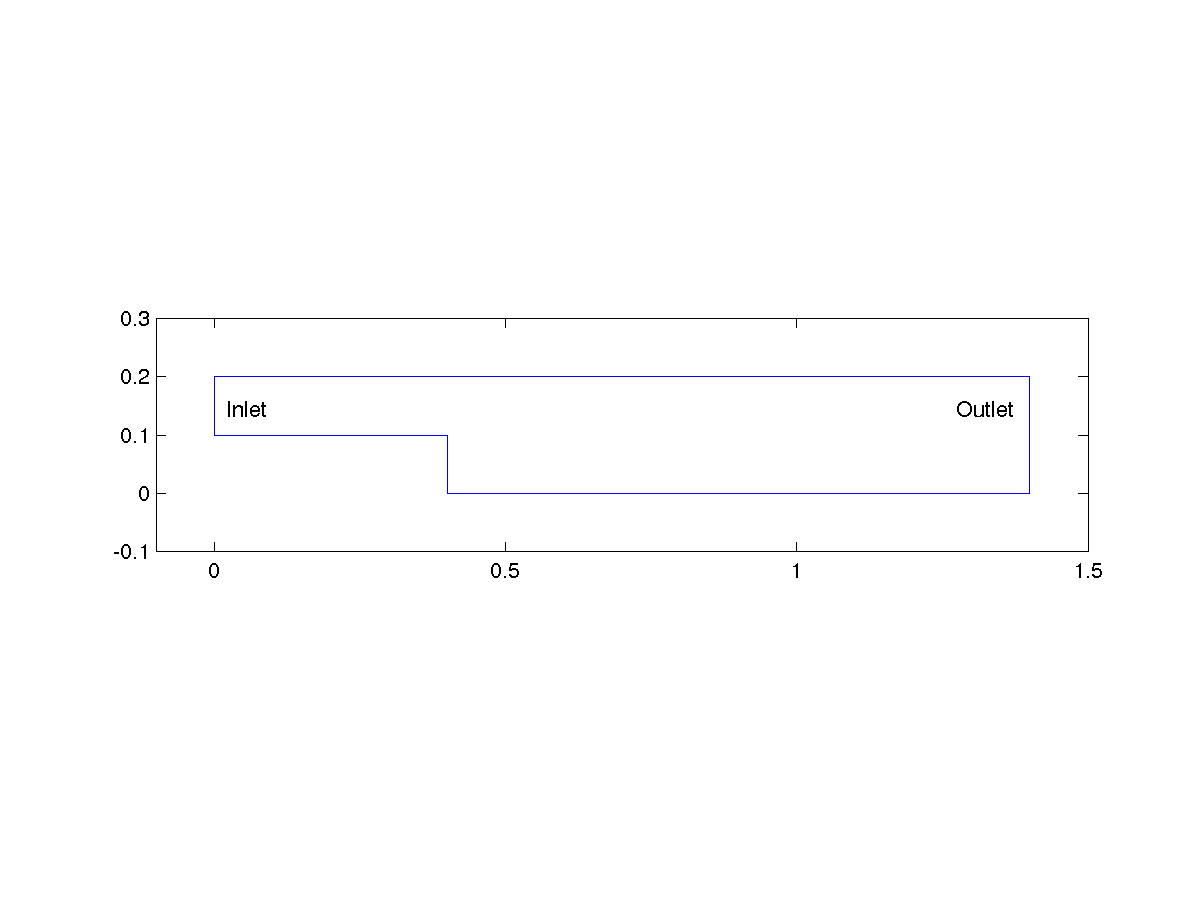
\includegraphics[height=80mm]{step_geometry.png}
\caption{Step.}\label{fg:step_geometry}
\end{figure}

\begin{table}[h]
\caption{Material parameters.}
\label{tb:matpam}
\begin{center}
\begin{tabular}{ll} \hline
parameter  & value \\ \hline
viscosity & 16.7e-6 Ns/m$^{2}$  \\
heat conductivity & 0.026 W/(m$\cdot$K) \\
heat capacity & 1.01e3 J/(kg$\cdot$K) \\
specific heat ratio & 1.4        \\
reference pressure & 1e5 Pa      \\ \hline
\end{tabular}
\end{center}
\end{table}


\subsection*{Solution procedure}

\begin{flushleft}

The mesh consists of 500 rectangular elements and it is constructed using ElmerGrid with the following command

\ttbegin
ElmerGrid 1 2 mesh.grd
\ttend

This command creates the sub-directory {\tt mesh} which contains the Elmer mesh files.

\ttbegin
Header
  Mesh DB "." "mesh"
  Include Path ""
  Results Directory ""
End
\ttend

The simulation uses 2D Cartesian geometry and the problem is solved in steady state using no more than twenty steady state iterations.

\ttbegin
Simulation
  Coordinate System =  Cartesian 2D
  Coordinate Mapping(3) = 1 2 3
  Simulation Type = Steady
  Steady State Max Iterations = 20
  Solver Input File = "compress_step.sif"
  Post File = "compress_step.vtu"
  Output File = "compress_step.dat"
End
\ttend

The solvers are coupled and therefore the convection is computed. 

\ttbegin
Equation 1
  Navier-Stokes = True
  Heat Equation = True
  Convection = "Computed"
End
\ttend

Due to the simplicity of the model only one body is needed.

\ttbegin
Body 1
  Equation = 1
  Material = 1
  Initial Condition = 1
End
\ttend

Our intention is to model compressible flow and that is why we have to set the value ''Perfect Gas'' for the keyword {\tt Compressibility Model}. Furthermore, because perfect gas model has been chosen the settings {\tt Reference Pressure} and {\tt Specific Heat Ratio} must also be given. The Navier-Stokes equation also needs the value of viscosity and the heat equation needs the values of heat capacity and heat conductivity.

\ttbegin
Material 1
  Compressibility Model = String "Perfect Gas"
  Reference Pressure = 1e5
  Specific Heat Ratio = 1.4
  Viscosity = 16.7e-6
  Heat Conductivity = 0.026
  Heat Capacity = 1.01e3
End
\ttend

For the initial value of temperature we have chosen 300 K.

\ttbegin
Initial Condition 1
  Temperature = 300
End
\ttend

The Navier-Stokes equation is solved first. Here we give the linear system solver and convergence criterions for linear, nonlinear and steady state solution of the Navier-stokes equation. Note that we are solving for the compressible Navier-stokes equation and that is why a bubble function formulation is used for stabilization of the equation.


\ttbegin
Solver 1
  Equation = "Navier-Stokes"
  Linear System Solver = "Iterative"
  Linear System Iterative Method = "BiCGStab"
  Linear System Max Iterations = 500
  Linear System Convergence Tolerance = 1.0e-08
  Linear System Abort Not Converged = True
  Linear System Preconditioning = "ILU2"
  Linear System Residual Output = 1
  Steady State Convergence Tolerance = 1.0e-05
  Bubbles = Logical True
  Nonlinear System Convergence Tolerance = 1.0e-05
  Nonlinear System Max Iterations = 1
  Nonlinear System Newton After Iterations = 3
  Nonlinear System Newton After Tolerance = 1.0e-02
  Nonlinear System Relaxation Factor = 1
End
\ttend

The corresponding parameters for the solver of the heat equation are defined in the following solver section.

\ttbegin
Solver 2
  Equation = "Heat Equation"
  Variable = "Temperature"
  Linear System Solver = "Iterative"
  Linear System Iterative Method = "BiCGStab"
  Linear System Max Iterations = 350
  Linear System Convergence Tolerance = 1.0e-08
  Linear System Preconditioning = "ILU0"
  Linear System Residual Output = 1
  Steady State Convergence Tolerance = 1.0e-05
  Bubbles = Logical True
  Nonlinear System Convergence Tolerance = 1.0e-05
  Nonlinear System Max Iterations = 1
  Nonlinear System Newton After Iterations = 3
  Nonlinear System Newton After Tolerance = 1.0e-02
  Nonlinear System Relaxation Factor = 1
End
\ttend

Finally, the boundary conditions are specified. There are three sets of boundary conditions, so three {\tt Boundary Condition} sections are needed. The first one is used to prescribe the boundary conditions in the inlet region. Note that we have defined the x-velocity and temperature as a variable of y-coordinate. 
This is done by setting different values for the x-velocity and temperature 
(the numerical values of the second column between the words {\tt Real} and {\tt End})
in the different y-points
(the numerical values of the first column between words {\tt Real} and {\tt End})
of the inlet region.
This kind of procedure prevents singularities from occurring in the corner points of the inlet region. In addition, this kind of definition is more realistic than a constant condition, in which the values of the x-velocity and temperature remain the same in the whole inlet region. 

\ttbegin
Boundary Condition 1
  Target Boundaries = 1
  Velocity 1 = Variable Coordinate 2
    Real 
      0.1    0
      0.15   0.02
      0.2    0
    End

  Velocity 2 = 0
  Temperature = Variable Coordinate 2
    Real 
      0.1    300
      0.15   350
      0.2    300
    End
End
\ttend

After the rest of the boundary conditions have been defined the problem is ready to solve.

\ttbegin
Boundary Condition 2
  Target Boundaries = 2
  Velocity 2 = 0
End

Boundary Condition 3
  Target Boundaries = 3
  Velocity 1 = 0
  Velocity 2 = 0
  Temperature = 300
End
\ttend

\subsection*{Results}

Figure \ref{fg:comp_step_temp} presents the temperature distribution of the step in steady state. The maximum and minimum values of x- and y-velocities are also given as a result and they are shown in Table \ref{tb:velocities}.

\begin{figure}[h]
\centering
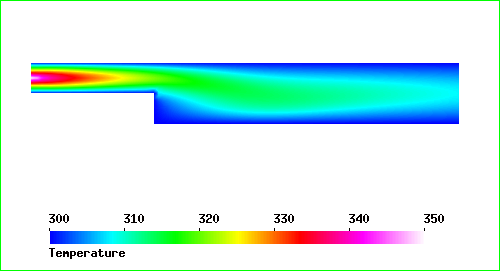
\includegraphics[height=80mm]{comp_step_temp.png}
\caption{Step.}\label{fg:comp_step_temp}
\end{figure}

\begin{table}[h]
\caption{Computed velocities.}
\label{tb:velocities}
\begin{center}
\begin{tabular}{ll} \hline
velocity  & value \\ \hline
min x-velocity & -0.0014 m/s\\
min y-velocity & -0.0016 m/s        \\
max y-velocity & 0.0008 m/s      \\ \hline
\end{tabular}
\end{center}
\end{table}

\end{flushleft}

\vfill
